\chapter{考察}
本章では,その性能や回路スケールに影響を及ぼす要因や
遅延時間以外の設計選択肢について考察していく.
\section{遅延時間差の検知}
光レースロジック回路は図\ref{fig:ctrl}に示すように
コントロールと光伝搬出力信号のアレイ伝搬遅延時間を計測する部分とアレイからなるものを想定し,
本論文にて光レースロジックアレイを提案した.
光伝搬出力信号のアレイ伝搬遅延時間を計測する部分を検知部分と呼称し,
本節ではこの検知部分について考察する.

本提案の光レースロジックアレイは図\ref{fig:scorematrix_3}に示すスコアマトリクスを使用している.
この場合には,光伝搬出力信号の時間差は一つのセルの通過時間単位で変化する.
よって,検知部分では一つのセルの通過時間の差を検知できれば良い.
ゲート長が1$\mu m$の場合,一つのセルの通過時間は12.52psである.
デジタルカウンタを用いて遅延時間差を検知部分を構成すると,
カウンタを約80GHzで動作させなければならない.

また,使用するスコアマトリクスを変化させた場合も考える.
図\ref{fig:scorematrix_4}にスコアマトリクスの一例を示す.
\begin{figure}[t!]
\begin{center}
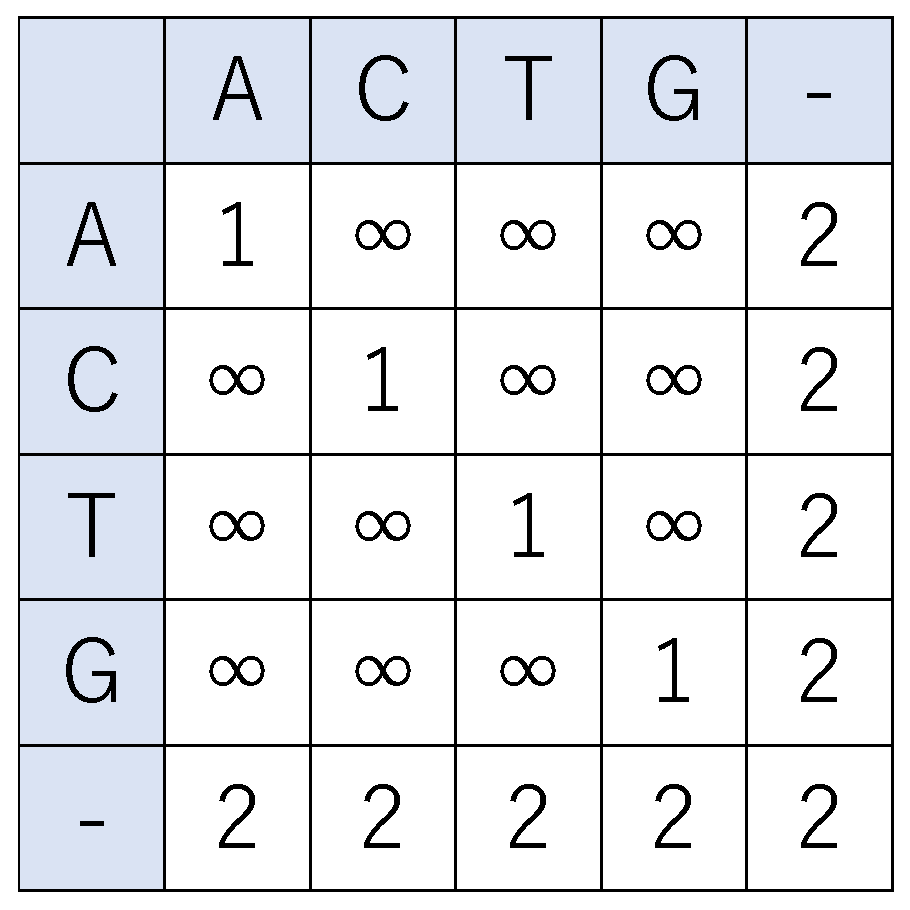
\includegraphics[keepaspectratio,scale=0.4]{fig/5/scorematrix_4.eps}
\caption{スコアマトリクスの一例}
\label{fig:scorematrix_4}
\end{center}
\end{figure}
このスコアマトリクスでは,図\ref{fig:scorematrix_3}に示すスコアマトリクス
とは違い,欠損・挿入に対応するギャップスコアが2となっている.
本提案の光レースロジックアレイでは,光遅延素子で発生させる遅延時間を
光スイッチを通過する際の伝搬遅延時間の倍と
することで図\ref{fig:scorematrix_4}に示す
スコアマトリクスに基づく配列アラインメントスコアを求めることができる.
この場合,光伝搬出力信号の時間差は光スイッチの通過時間単位で変化し,
光スイッチの通過時間はそのゲート長にて決定される.
ゲート長の最小加工寸法が1$\mu m$である時,
光スイッチを通過する際の遅延時間は10$fs$であり,
光遅延素子にて発生させる遅延時間は20$fs$である.
検知部分では10$fs$の遅延時間差を検知できなければならない.
もしデジタルカウンタを用いて遅延時間差を検知部分を構成するとすると,
カウンタを100THzで動作させなければならない.

その様な動作周波数でデジタルカウンタを動作させることは不可能である.
よって,検知部分をデジタルカウンタで構成した場合には,
検知部分が光レースロジック回路の性能を律速する要因となる.

光レースロジックアレイをもって光伝搬信号の遅延時間に情報を付与できることは
本研究の検証によって明らかになった.
光レースロジックアレイの光速での計算能力を活かす
検知部分の構成を考えることが必要である.

\section{雑音の影響}
光伝搬信号の特徴として,伝搬するに従って雑音が蓄積していくというものがある.
本節では,光伝搬信号の強度や遅延時間に影響を与える雑音について考察していく.
\subsection{光伝搬信号強度に影響を与える雑音}
ここでは光伝搬信号強度に影響を与える雑音を考える.
光スイッチの漏れ率$\beta$はスイッチがオフ動作の際に光伝搬信号を遮断しきれずに,
どの程度出力へ漏れ出すかを表す漏れ率である.
遮断しきれずに漏れ出した光伝搬信号は次のセルへと伝搬し光アンプにて増幅され,
雑音信号のように振る舞う.
具体例として,配列長N=2の光レースロジックアレイの出力を考える.
光レースロジックアレイのスイッチ状態が図\ref{fig:all_switch_12}の状態を取る時,
1つのセルの伝搬遅延時間を$1ns$とすると,
最初に光伝搬出力信号が検出されるのは入力から$4ns$後と想定される.
図\ref{fig:off_beta}に光レースロジックアレイに光伝搬信号を入力してからの
様子を示す.
赤く示した部分が光伝搬信号が伝搬している経路と到達する素子である.
青く示した部分は光スイッチで漏れ出した信号が伝搬する経路である.
光伝搬信号入力から$2ns$後と$3ns$後に光スイッチで漏れ出した
光伝搬信号が受光器まで到達する.
この光スイッチで漏れ出した光伝搬信号の強度が受光器の最小受光感度
以上になると,本来想定された伝搬遅延時間以外のタイミングで
出力信号を検出してしまう.
\begin{figure}[t!]
\begin{center}
\subfigure[光伝搬信号入力から$1ns$後]{
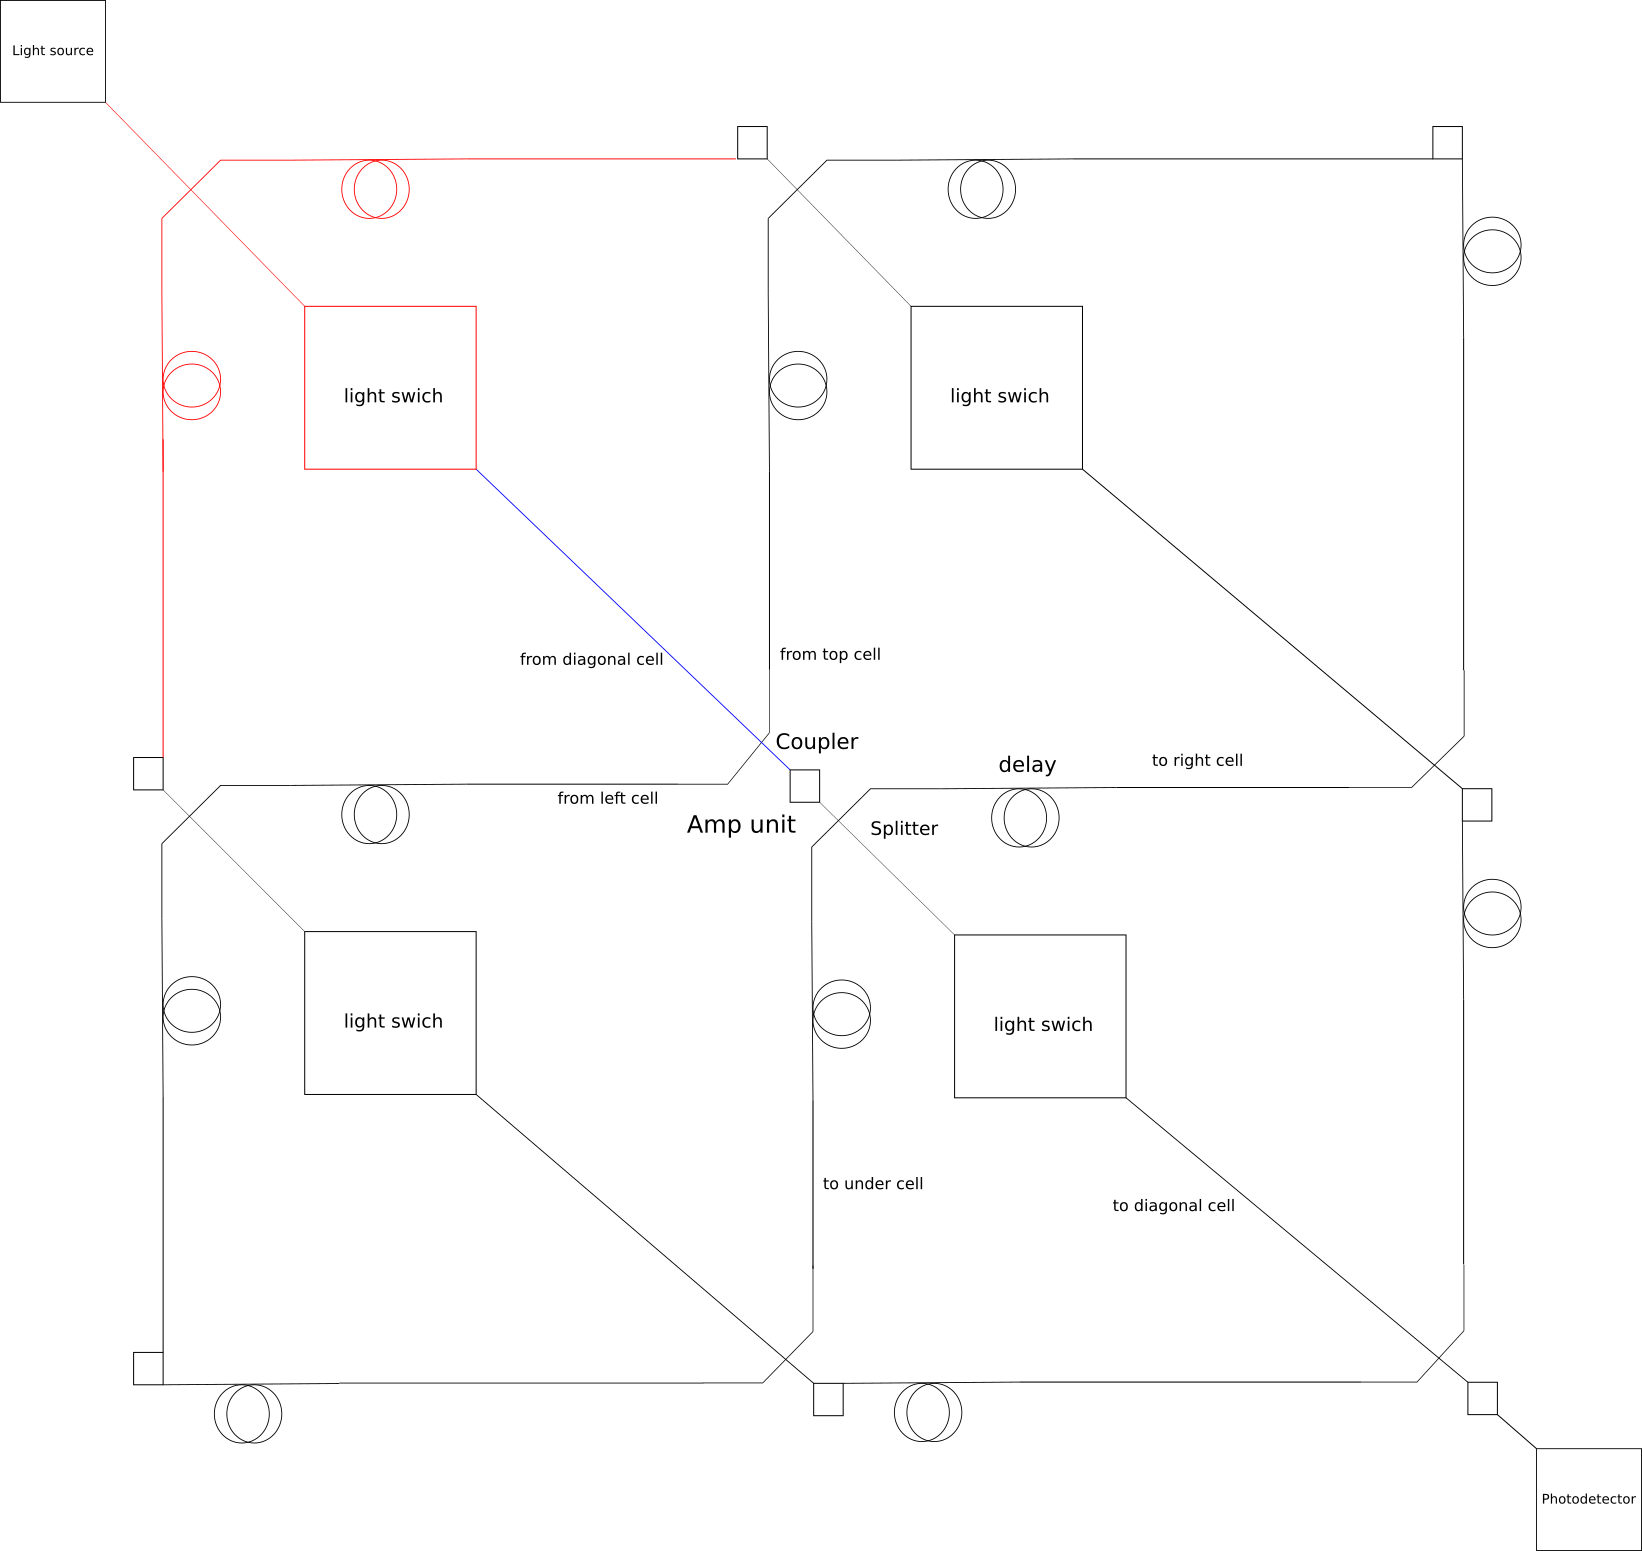
\includegraphics[keepaspectratio,scale=0.15]{fig/5/lightracelogic_N_2_beta1.png}}
\subfigure[光伝搬信号入力から$2ns$後]{
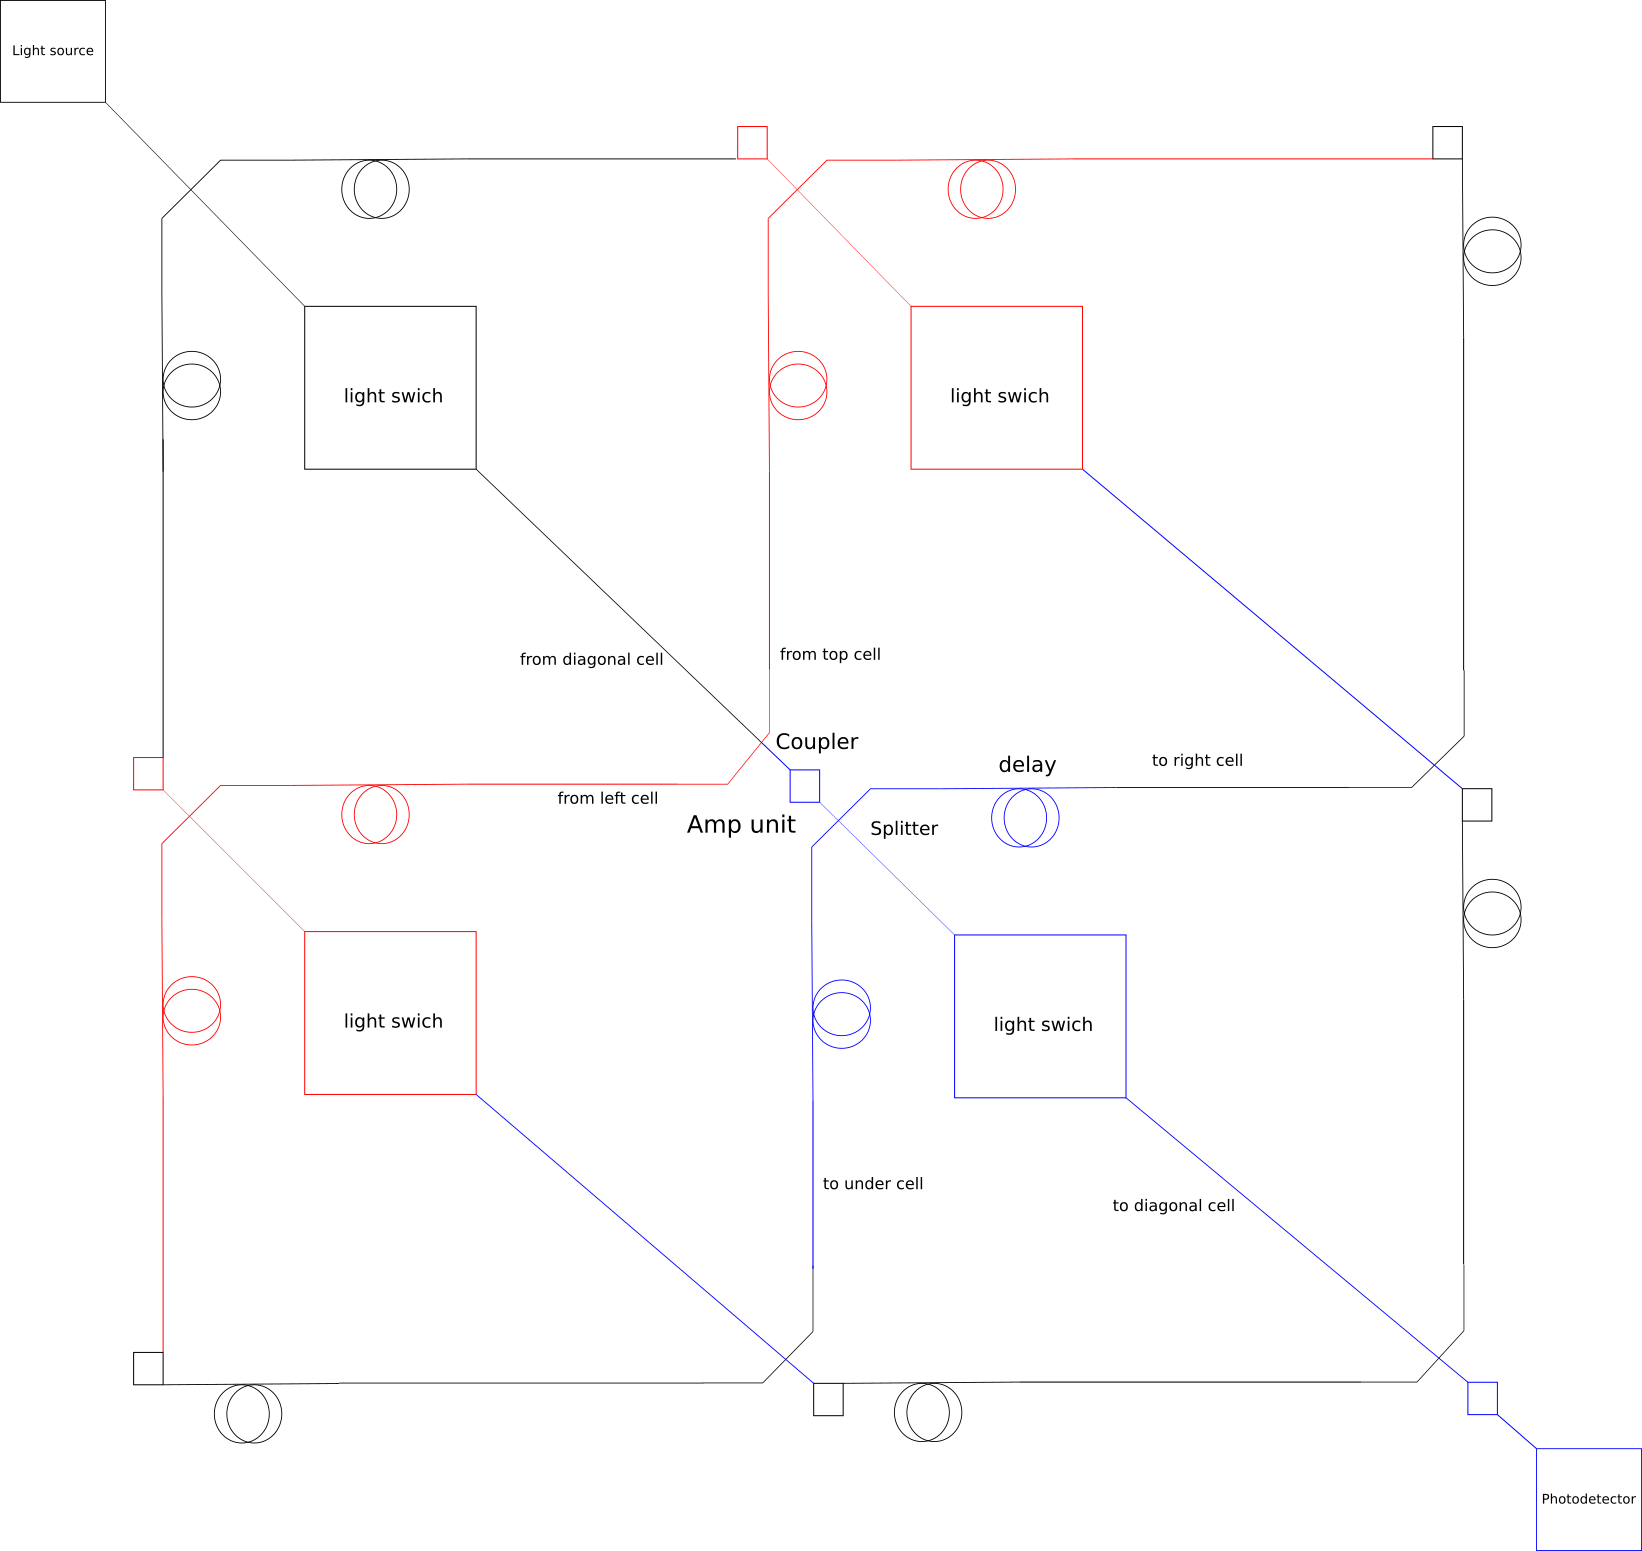
\includegraphics[keepaspectratio,scale=0.15]{fig/5/lightracelogic_N_2_beta2.png}}\\
\subfigure[光伝搬信号入力から$3ns$後]{
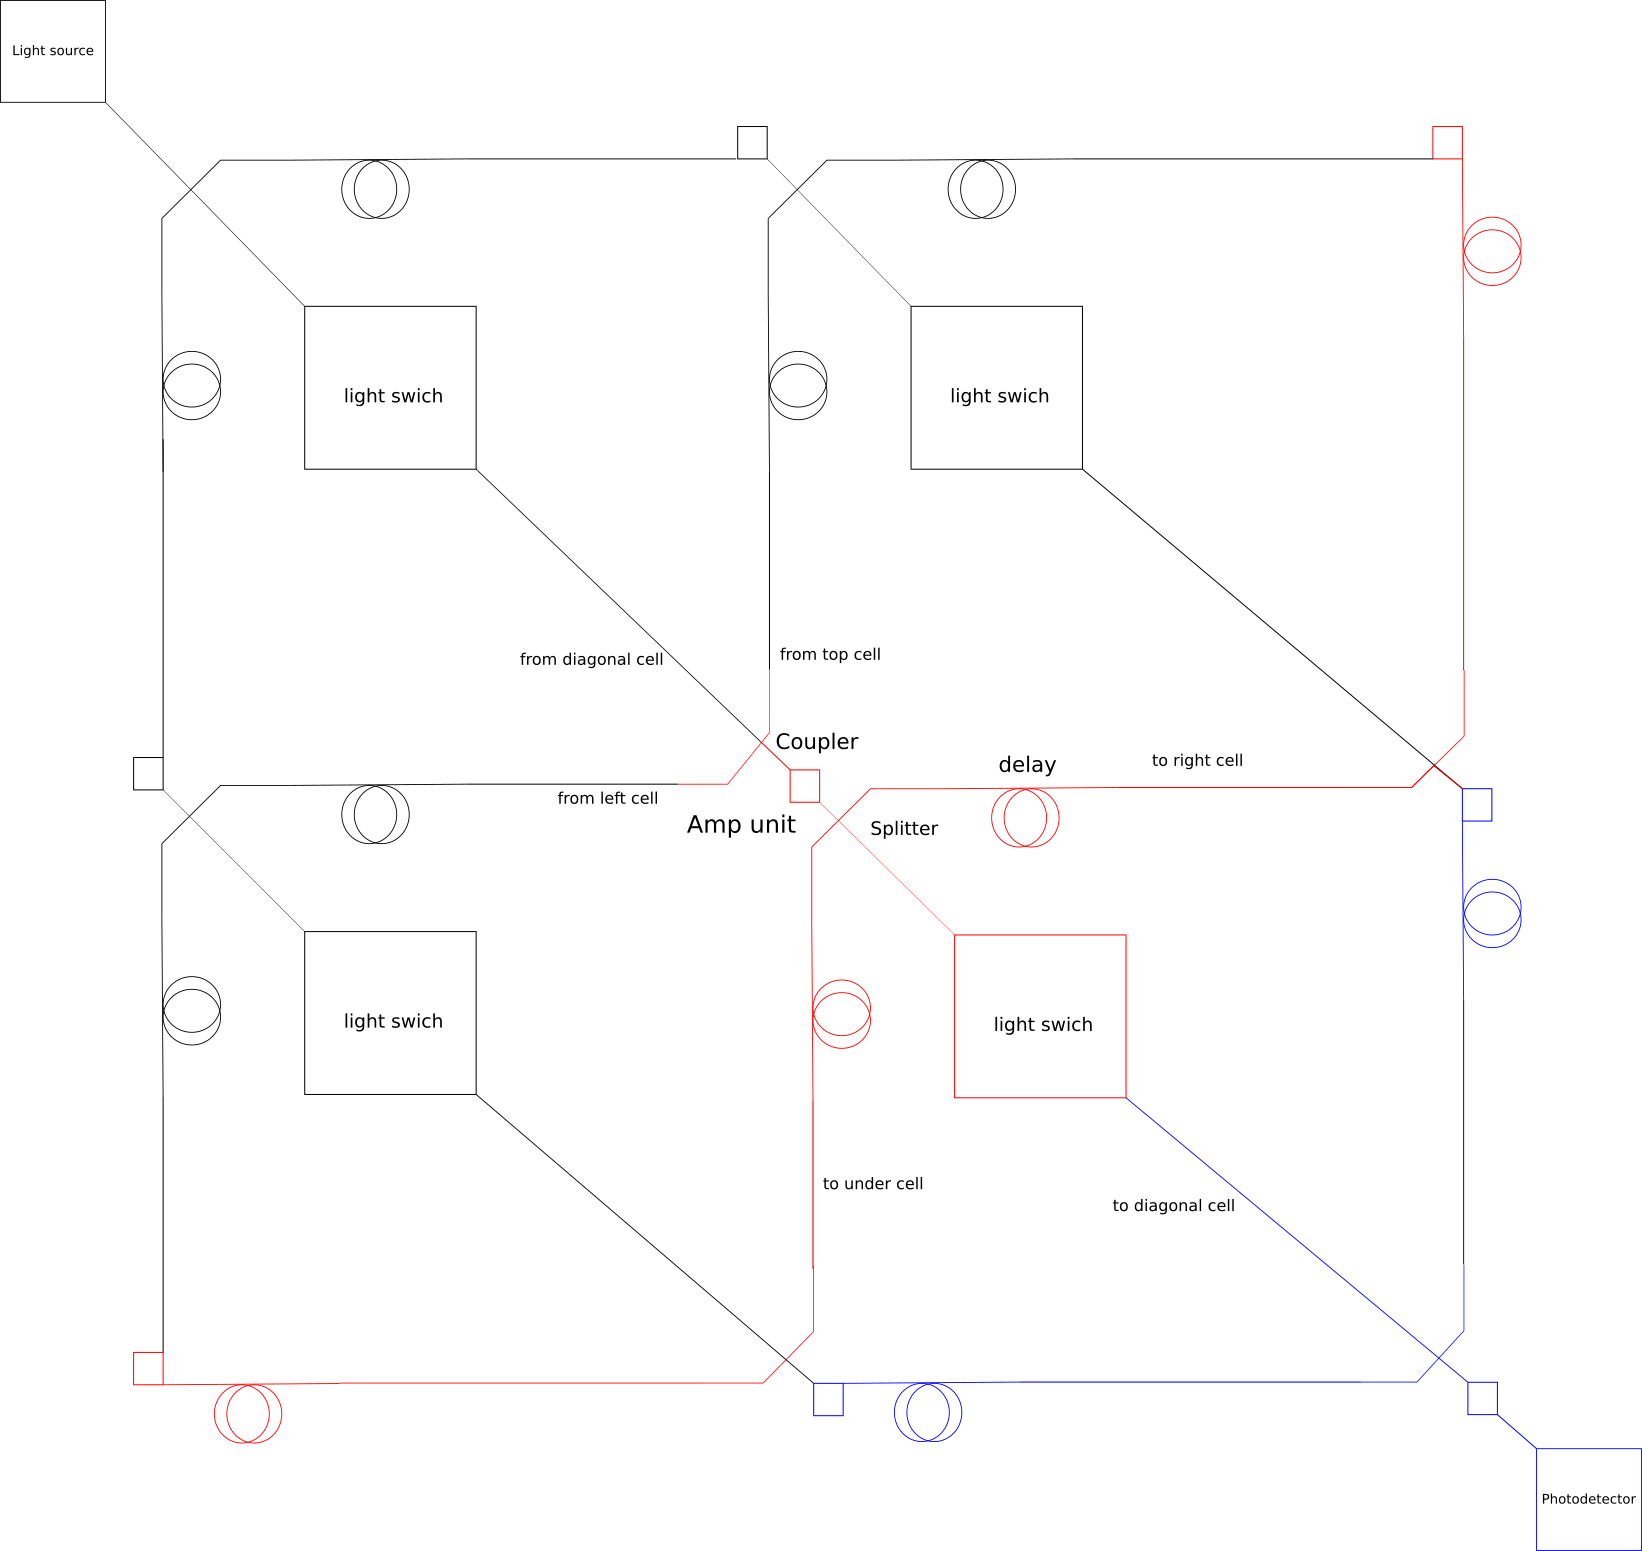
\includegraphics[keepaspectratio,scale=0.15]{fig/5/lightracelogic_N_2_beta3.png}}
\subfigure[光伝搬信号入力から$4ns$後]{
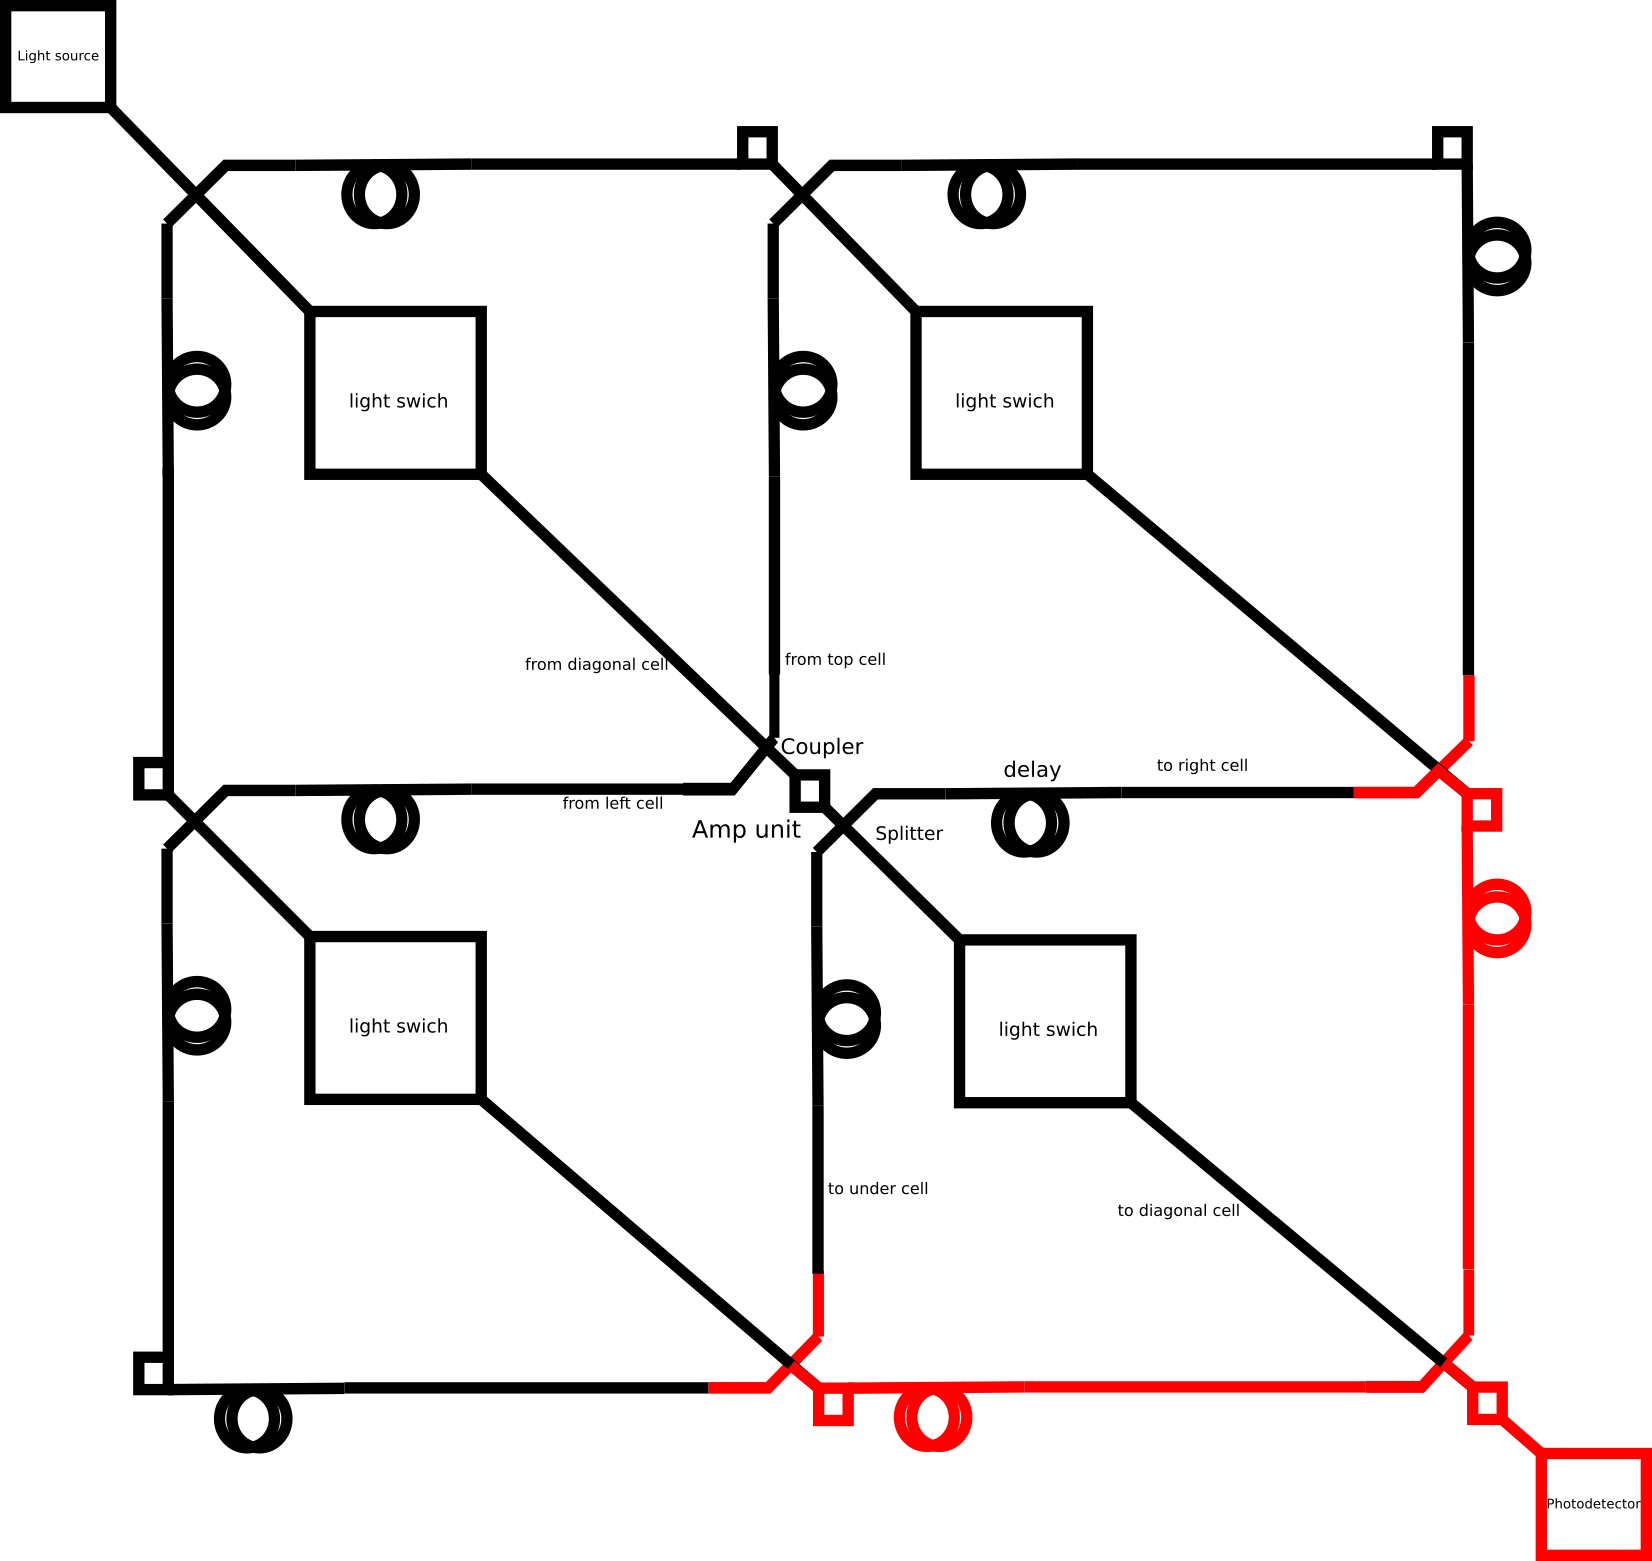
\includegraphics[keepaspectratio,scale=0.15]{fig/3/lightracelogic_N_2_on4.png}}\\
\caption{光スイッチの漏れを考慮した光レースロジックアレイの挙動}
\label{fig:off_beta}
\end{center}
\end{figure}

また,光スイッチにはスイッチがオン動作の際にスイッチから回路外へ光伝搬信号が
どの程度漏れ出すかを表す漏れ率$\alpha$が存在する.
この漏れ率$\alpha$は光スイッチの製造ばらつきや光スイッチの制御信号の揺らぎによって
その値にばらつきが生じる.
光結合器,光分配器,光遅延素子での損失に関しても,
製造ばらつきなどによってその値にばらつきが生じる.
4.2.3項で述べたように,光レースロジックアレイの機能を担保するためには
アレイからの出力の最小値が受光器によって検出可能な強度でなければならない.
漏れや損失のばらつきによってアレイからの出力の最小値が揺らぎ,
これを考慮して光レースロジック アレイの機能を担保するための光源・アンプの消費電力を
設定しなければならないことが考えられる.

上記2つの光伝搬信号強度に関する雑音によって
配列長Nのスケーリングに影響を及ぼす可能性がある.

\subsection{光伝搬信号の遅延時間に影響を与える雑音}
ここでは光伝搬信号の遅延時間に影響を与える雑音を考える.
光デバイスの伝搬遅延時間は製造ばらつきを主な要因とする誤差が存在する.
提案した非同期型の光レースロジック アレイでは,
光伝搬信号の遅延時間の誤差も伝搬するに従って蓄積されていく.
これにより,とある配列の組み合わせにおいて想定される光伝搬信号の出力のタイミングと
実際の出力のタイミングに差が生じることが考えられる.

この遅延時間の誤差は,スコア1の重みをどの程度の遅延時間と定めるかによってその影響が変化する.
また,製造ばらつきを要因とする誤差はチューニングをすることによって
ある程度吸収が可能であると推察する.

遅延時間のばらつきが配列長Nのスケーリングにどう影響を及ぼすのかを考えていく必要がある.

\section{遅延時間以外の設計選択肢}
これまで,回路からの出力信号の遅延時間というアナログ量にとある情報付加するレースロジックと
情報媒体にアナログ量を取り扱う光デバイスの親和性に着目してきた.
光デバイスが取り扱えるアナログ量は遅延時間だけではなく,
位相,信号強度などが存在する.
レースロジックは伝搬信号に遅延時間を重みとして付与して動的計画法によって求められる最適化問題を解くという考えである.
光デバイスを用いることで,その考えを発展させ,
光伝搬信号の位相変化や強度変化を重みとして付与して動的計画法によって求められる最適化問題を解くものを
考えることができる.
今回はその中でも光伝搬信号の位相に着目して述べる.

設計選択肢として位相を選択する場合,光レースロジックアレイからの光出力信号の位相が
とある情報を持つ計算結果となる.
位相は$0〜2\pi$の間の値を取り,
各パスでの重み付けは位相シフタなどを用いて位相をずらすことによって行う.
光レースロジックアレイを伝搬した光出力信号の位相を
位相計測器などを用いて計測する.
配列アラインメントスコアの例を用いて述べると,
スコアマトリクスに基づく位相変化を光伝搬信号に付与し,
光出力信号の位相が配列が完全に一致する場合において推定される光出力信号の位相と
どの程度差があるかが配列アラインメントスコアに相当する.

設計選択肢に位相を選択した場合,光出力信号への重み付けに用いるスコアに負の値を用いることができるという特徴がある.
配列アラインメントに用いられるスコアマトリクスには負の値を含むものも存在する.
しかし,遅延時間を重みに選択した場合にはこの負のスコアを付与することができない.
負の値を含むスコアマトリクスを使用する場合には,
スコアマトリクスの値全体に対してバイアスをかける事で
負の値を正の値へと変換することが必要になる.
位相を重み付けに選択した場合,負のスコアを付与することが可能になる.
図\ref{fig:isou}に位相を用いて負のスコアを付与する例を示す.
\begin{figure}[t!]
\begin{center}
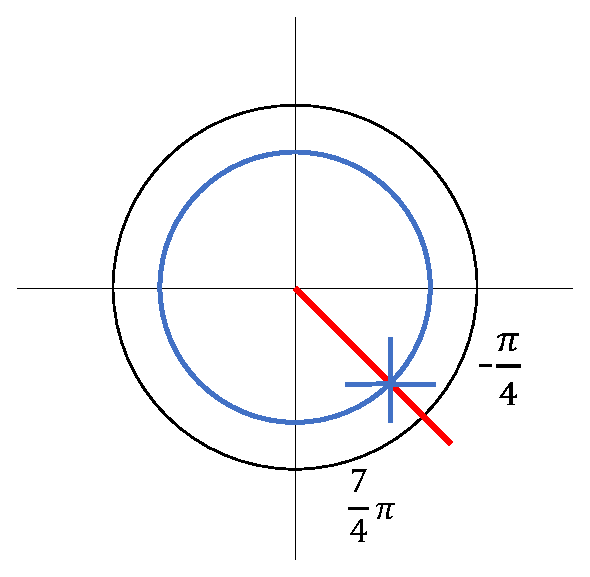
\includegraphics[keepaspectratio,scale=0.5]{fig/5/isou.eps}
\caption{位相を用いて負のスコアを付与する例}
\label{fig:isou}
\end{center}
\end{figure}
$-\frac{\pi}{4}$の重み付けをする場合,位相を$\frac{7}{4}\pi$ずらすことによってそれを表現できる.

位相を重み付けに選択した場合,
光信号の位相計測器の分解能によって重み付けに用いる位相差の最小単位が決定される.
よって,位相計測器の性能が配列長Nのスケーリングに影響を及ぼすことが考えられる.
また,光レースロジックアレイからの光出力信号の位相が
負の値の場合や$2\pi$を超える場合にはそれを計測できない.
更に,違う位相の光伝搬信号同士は干渉するので,
光レースロジック アレイ内を伝搬中に干渉しないようにする,
もしくは干渉することを踏まえた設計をしなければならない.
実装を検討する際には,これらをどう取り扱うかが問題となる.
